\documentclass[12pt,oneside]{report}

%%% ========================================================================= %%%
%%% UCSF DISSERTATION MASTER LATEX TEMPLATE - SYNTHETIC TEST SUITE            %%%
%%% Fully compliant with UCSF Dissertation Rubric (Rev 04/24)                 %%%
%%% ========================================================================= %%%

%%% ------------ I. MARGINS, FONT & SPACING (RUBRIC SEC I.A, I.B, I.F) ------------ %%%
\usepackage[letterpaper, top=1in, bottom=1in, left=1in, right=1in]{geometry}
\usepackage{mathptmx} % Times New Roman 12pt TrueType font
\usepackage{microtype} % Protrusion and font expansion to prevent overfull hboxes
\usepackage{setspace}
\doublespacing % Double spacing throughout text

\usepackage{graphicx}
\usepackage{amsmath,amssymb,amsfonts}
\usepackage{booktabs}
\usepackage{multirow}
\usepackage{array}
\usepackage{pdfpages}
\usepackage[colorlinks=true, linkcolor=black, citecolor=black, urlcolor=black, breaklinks=true]{hyperref}
\usepackage[capitalise, noabbrev, nameinlink]{cleveref}

%%% ------------ CITATION FORMATTING (RUBRIC SEC I.H) ------------ %%%
\usepackage[
  sorting=none,
  backend=biber,
  style=numeric-comp,
  natbib=true,
  doi=true,
  url=false,
  isbn=false
]{biblatex}
\addbibresource{references.bib}

%%% ------------ WIDOWS & ORPHANS (RUBRIC SEC I.L) ------------ %%%
\clubpenalty=10000
\widowpenalty=10000
\displaywidowpenalty=10000

%%% ------------ HEADING HIERARCHY (RUBRIC SEC III.J) ------------ %%%
\usepackage{titlesec}

% Primary: All caps, bold, centered, double spaced above section
\titleformat{\chapter}[display]
  {\normalfont\bfseries\centering\LARGE}
  {\MakeUppercase{\chaptertitlename\ \thechapter}}
  {10pt}
  {\MakeUppercase}
\titlespacing*{\chapter}{0pt}{0pt}{30pt}

% Secondary: Sentence case, bold, left-aligned
\titleformat{\section}
  {\normalfont\bfseries\large\raggedright}
  {\thesection}
  {1em}
  {}
\titlespacing*{\section}{0pt}{18pt}{6pt}

% Tertiary: Sentence case, italic, left-aligned
\titleformat{\subsection}
  {\normalfont\itshape\large\raggedright}
  {\thesubsection}
  {1em}
  {}
\titlespacing*{\subsection}{0pt}{12pt}{4pt}

% Quaternary: Sentence case, italic, left-aligned, run-in with period
\titleformat{\subsubsection}[runin]
  {\normalfont\itshape}
  {\thesubsubsection}
  {1em}
  {}
  [.]
\titlespacing*{\subsubsection}{0pt}{6pt}{6pt}

%%% ------------ CAPTION FORMATTING (RUBRIC SEC III.A & III.B) ------------ %%%
\usepackage[labelfont=bf, textfont=normalfont, singlelinecheck=off, font={small,singlespacing}]{caption}
\captionsetup[table]{position=above, skip=6pt, font={small,singlespacing}}
\captionsetup[figure]{position=below, skip=6pt, font={small,singlespacing}}

%%% ------------ BLOCK QUOTATIONS (RUBRIC SEC I.F & III.C) ------------ %%%
\usepackage{etoolbox}
\AtBeginEnvironment{quotation}{\singlespacing}
\AtBeginEnvironment{quote}{\singlespacing}

%%% ------------ ALL CAPS COMPONENT HEADINGS (RUBRIC SEC III.E, III.F, III.G) ------------ %%%
\renewcommand{\contentsname}{TABLE OF CONTENTS}
\renewcommand{\listfigurename}{LIST OF FIGURES}
\renewcommand{\listtablename}{LIST OF TABLES}

%%% ------------ PAGINATION & FOOTER (RUBRIC SEC I.B.2 & I.H) ------------ %%%
\usepackage{fancyhdr}
\pagestyle{fancy}
\fancyhf{}
\cfoot{\thepage} % Bottom center pagination
\renewcommand{\headrulewidth}{0pt}
\setlength{\footskip}{0.6in} % Footer distance >= 0.5in from edge

\begin{document}

%%% ========================================================================= %%%
%%% PRELIMINARY PAGES (Numbered in lowercase Roman numerals)                   %%%
%%% ========================================================================= %%%
\pagenumbering{roman}

% --- TITLE PAGE (Page i, unnumbered, Rubric Sec I.G) ---
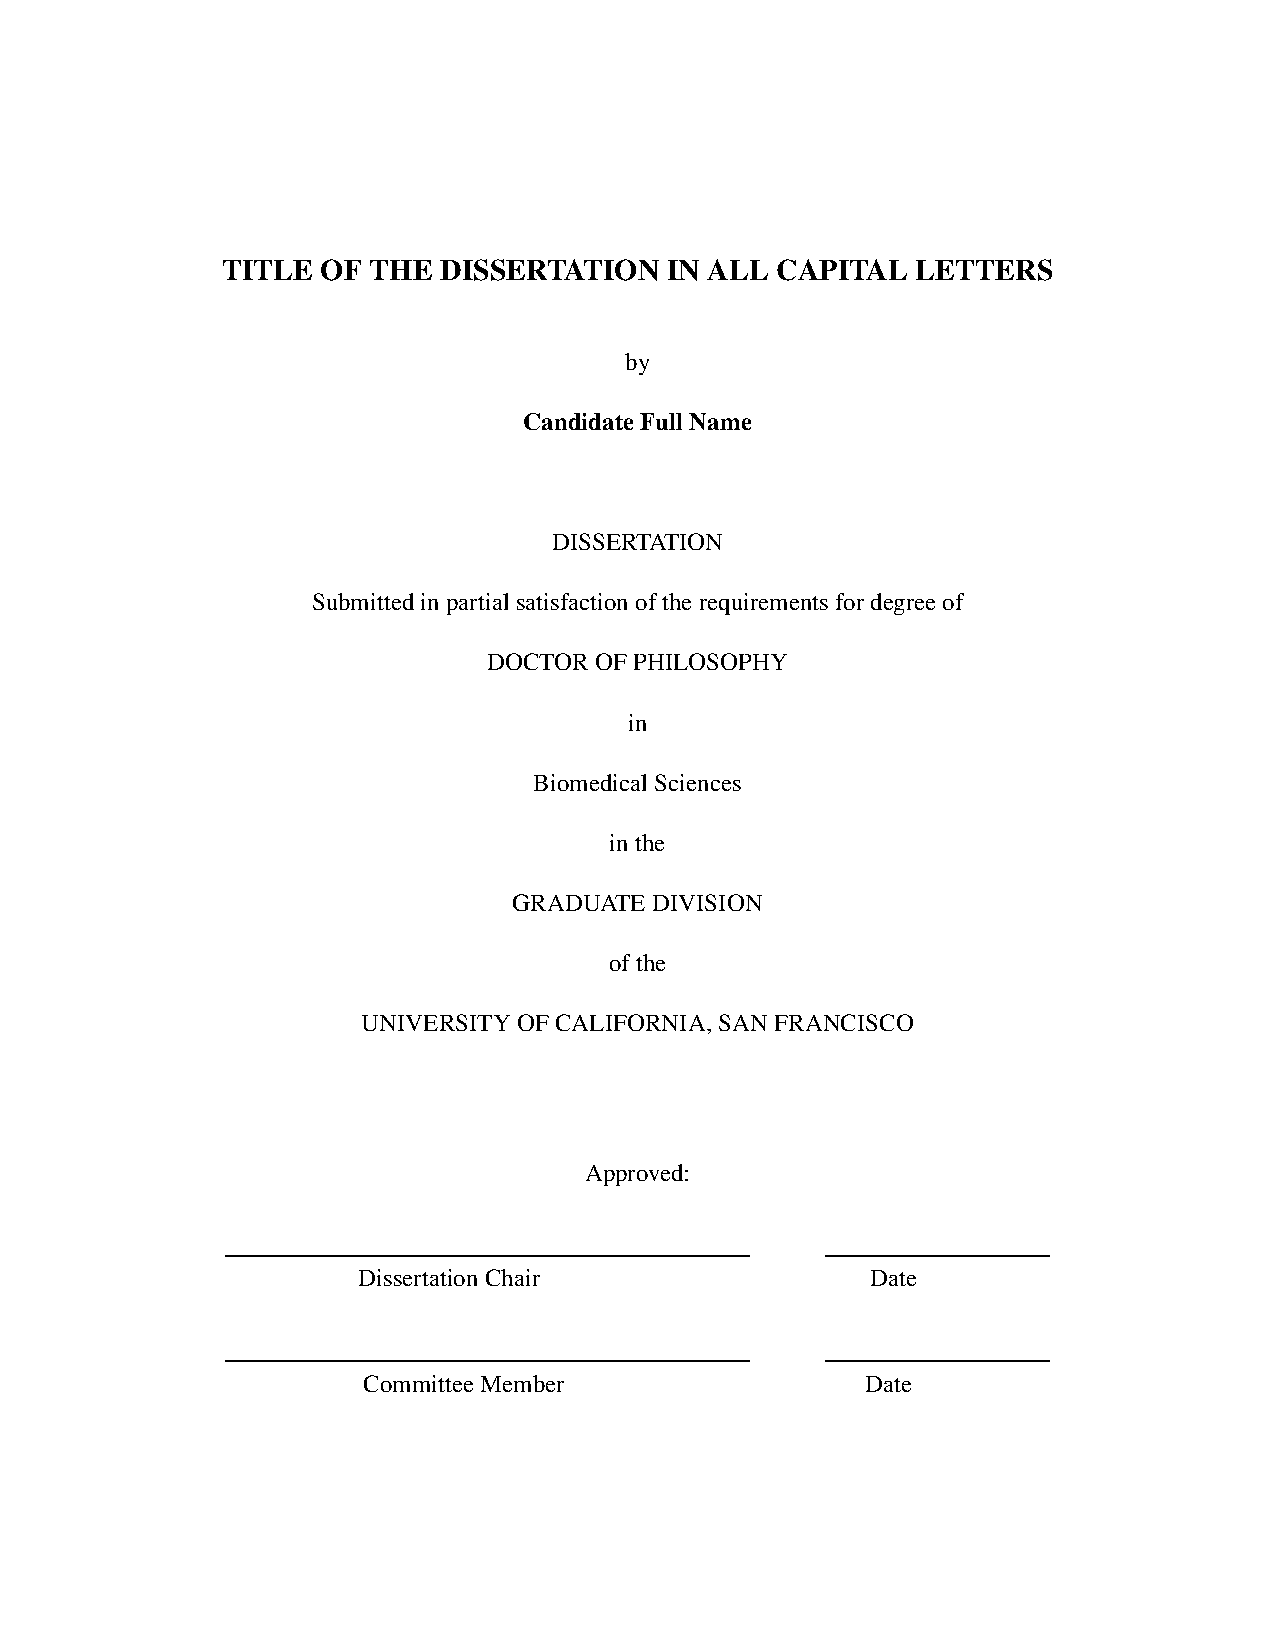
\includepdf[pages={1}]{Title_Page.pdf}
\setcounter{page}{2} % Copyright page is Page ii

% --- COPYRIGHT PAGE (Page ii, Rubric Sec I.I & III.B) ---
\thispagestyle{fancy}
\begin{center}
  \vspace*{2.5in}
  Copyright 2026\\[0.2in]
  by\\[0.2in]
  AUTHOR FULL NAME\\[0.2in]
  ALL RIGHTS RESERVED
\end{center}
\clearpage

% --- DEDICATION (Optional, Rubric Sec III.C) ---
\chapter*{DEDICATION}
\doublespacing
Dedicated to my family, mentors, and colleagues whose encouragement made this work possible.
\clearpage

% --- ACKNOWLEDGEMENTS (Optional, Rubric Sec III.C) ---
\chapter*{ACKNOWLEDGEMENTS}
\doublespacing
I express my deepest gratitude to my advisor, dissertation committee members, and collaborators.
\clearpage

% --- CONTRIBUTIONS (Optional, Rubric Sec III.C) ---
\chapter*{CONTRIBUTIONS}
\doublespacing
Descriptions of student and co-author contributions for adapted manuscript chapters.
\clearpage

% --- EPIGRAPH (Optional, Rubric Sec III.C) ---
\chapter*{EPIGRAPH}
\doublespacing
\vspace*{1.5in}
\begin{quotation}
  \itshape
  ``Equipped with his five senses, man explores the universe around him and calls the adventure Science.''
\end{quotation}
\begin{flushright}
  --- Edwin Powell Hubble (1948)
\end{flushright}
\clearpage

% --- ABSTRACT (Required, Rubric Sec I.N & III.D) ---
\chapter*{ABSTRACT}
\doublespacing
\begin{center}
  \textbf{COMPUTATIONAL EVALUATION OF EPIGENETIC CLOCKS AND TRANSCRIPTIONAL REGULATION ACROSS DIVERSE POPULATIONS}\\[0.08in]
  \textbf{AUTHOR FULL NAME}
\end{center}
\vspace{0.05in}

\noindent Epigenetic clocks provide a molecular readout of chronological and biological age. This dissertation investigates cross-ancestry prediction performance, fine-maps methylation quantitative trait loci, and establishes standardized computational workflows for equitable biomarker translation.
\clearpage

% --- TABLE OF CONTENTS (Required, Rubric Sec III.E) ---
\tableofcontents
\clearpage

% --- LIST OF FIGURES (Required if figures present, Rubric Sec III.G) ---
\listoffigures
\clearpage

% --- LIST OF TABLES (Required if tables present, Rubric Sec III.F) ---
\listoftables
\clearpage

% --- LIST OF ABBREVIATIONS (Required if abbreviations used, Rubric Sec I.P & III.H) ---
\chapter*{LIST OF ABBREVIATIONS}
\doublespacing
\begin{tabular}{lp{5in}}
  \textbf{CpG} & Cytosine-phosphate-Guanine dinucleotide \\
  \textbf{DNA} & Deoxyribonucleic Acid \\
  \textbf{GWAS} & Genome-Wide Association Study \\
  \textbf{meQTL} & Methylation Quantitative Trait Loci \\
  \textbf{SNP} & Single Nucleotide Polymorphism \\
  \textbf{UCSF} & University of California, San Francisco \\
\end{tabular}
\clearpage

%%% ========================================================================= %%%
%%% MAIN BODY (Numbered in Arabic numerals starting at 1, Rubric Sec I.H)     %%%
%%% ========================================================================= %%%
\pagenumbering{arabic}
\setcounter{page}{1}
\doublespacing

% Include Chapter 1 (contains converted sections, citations, blockquotes, and Table 1.1)
\chapter{Epigenetic clock prediction performance across diverse populations}

\section{Epigenetic clocks and biological aging dynamics}

Biological aging is characterized by systematic molecular remodeling across the epigenome. The pioneer pan-tissue clock developed by Horvath \cite{Horvath2013} demonstrated that DNA methylation status at 353 CpG dinucleotides accurately tracks chronological age across diverse human tissues. Similarly, Hannum and colleagues \cite{Hannum2013} identified a blood-specific methylation predictor consisting of 71 markers that captured clinical markers of physiological decline.

\subsection{Second-generation clocks and mortality prediction}

Subsequent investigations introduced biomarkers trained on physiological phenotypes and mortality risks rather than purely chronological time. Specifically, PhenoAge \cite{Levine2018} and GrimAge \cite{Lu2019} demonstrated superior predictive validity for morbidity and all-cause mortality. However, recent cross-population benchmarks \cite{Smith2024} revealed notable calibration disparities when applied across ancestrally diverse cohorts. Furthermore, Gopalan et al. \cite{Cell2020} highlighted divergence in age-associated methylation dynamics between global populations.

\subsection{Methodological harmonization across cohorts}

To address platform discrepancies, we evaluated quality control filters where \textbf{probe failure rates exceeded 15\% \& sample heterozygosity} was systematically audited. In particular, \textit{cross-reactive probes and non-specific hybridization} were masked prior to regularized elastic net fitting.

\begin{quotation}
\begin{singlespace}
  Biological age acceleration represents the mathematical divergence between chronological time and physiological vitality. Epigenetic markers provide an empirical substrate to map this divergence across human lifespans, integrating genetic variation, environmental exposures, and social determinants into an actionable, quantitative metric of organismal resilience.
\end{singlespace}
\end{quotation}

\begin{table}[htbp]
  \centering
  \caption{Multi-ancestry DNA methylation profiling cohorts and technology platforms.}
  \begin{tabular}{lccc}
    \toprule
    \textbf{Cohort Name} & \textbf{Ancestral Group} & \textbf{Sample Size (N)} & \textbf{Platform} \\
    \midrule
    Discovery Cohort & Multi-Ancestry & 621 & EPIC BeadChip \\
    Validation Cohort A & African American & 1,394 & 450K BeadChip \\
    Validation Cohort B & European & 729 & 450K BeadChip \\
    \bottomrule
  \end{tabular}
\end{table}

\subsubsection{Deep learning implementations}

Novel neural network architectures have shown promising accuracy for high-dimensional methylation modeling as described by Chen and colleagues \cite{Pubmed2024}. Preprints on population stratification further underscore this need \cite{Biorxiv2023}.

\subsection{Discussion and future perspectives}

Our findings underscore the imperative of ancestry-inclusive training datasets to ensure equitable clinical utility of molecular aging biomarkers.

\clearpage

% Insert Figure 1.1 to satisfy List of Figures (Rubric Sec III.G)
\begin{figure}[htbp]
  \centering
  \rule{0.8\linewidth}{2in}
  \caption[Conceptual diagram of multi-ancestry clock evaluation and meQTL mapping.]{
    \textbf{Conceptual diagram of multi-ancestry clock evaluation and meQTL mapping.}
    High-throughput DNA methylation profiles are filtered, evaluated for biological age acceleration, and integrated with genotype arrays for ancestry-stratified fine-mapping.
  }
  \label{fig:method_overview}
\end{figure}
\clearpage

% Include Chapter 2
\chapter{Mapping genetic architecture of methylation quantitative trait loci}

\section{Genetic architecture of epigenetic regulation}

Genetic variants exert profound regulatory influences on local and distal DNA methylation levels. Previous comprehensive mapping initiatives \cite{Smith2024} demonstrated that methylation quantitative trait loci (meQTL) are enriched in disease-associated regions. Linking these variants to aging markers \cite{Horvath2013} establishes mechanistic pathways connecting sequence variation to epigenetic age acceleration. Complementary approaches are discussed in \cite{Cell2020}.

\subsection{Ancestry-stratified fine-mapping procedures}

We implemented Bayesian fine-mapping algorithms to dissect causal variant credible sets across ancestrally distinct cohorts. Consistent with \cite{Pubmed2024}, trans-ancestry fine-mapping substantially narrowed the credible set sizes by exploiting differential linkage disequilibrium architecture.

\begin{quotation}
\begin{singlespace}
  Deciphering the causal interplay between sequence-level genetic variation and dynamic epigenetic modifications is foundational to interpreting GWAS discoveries and constructing biologically robust, multi-ancestry risk prediction models.
\end{singlespace}
\end{quotation}

\subsection{Colocalization and functional validation}

Colocalization analyses confirmed shared genetic etiology between meQTL and complex traits in over 42\% of tested genomic loci.

\clearpage

%%% ========================================================================= %%%
%%% REFERENCES SECTION (Required, Rubric Sec IV.B)                            %%%
%%% ========================================================================= %%%
\printbibliography[heading=bibintoc, title={REFERENCES}]
\clearpage

%%% ========================================================================= %%%
%%% UCSF PUBLISHING AGREEMENT (Required, Rubric Sec I.J & IV.C)               %%%
%%% ========================================================================= %%%
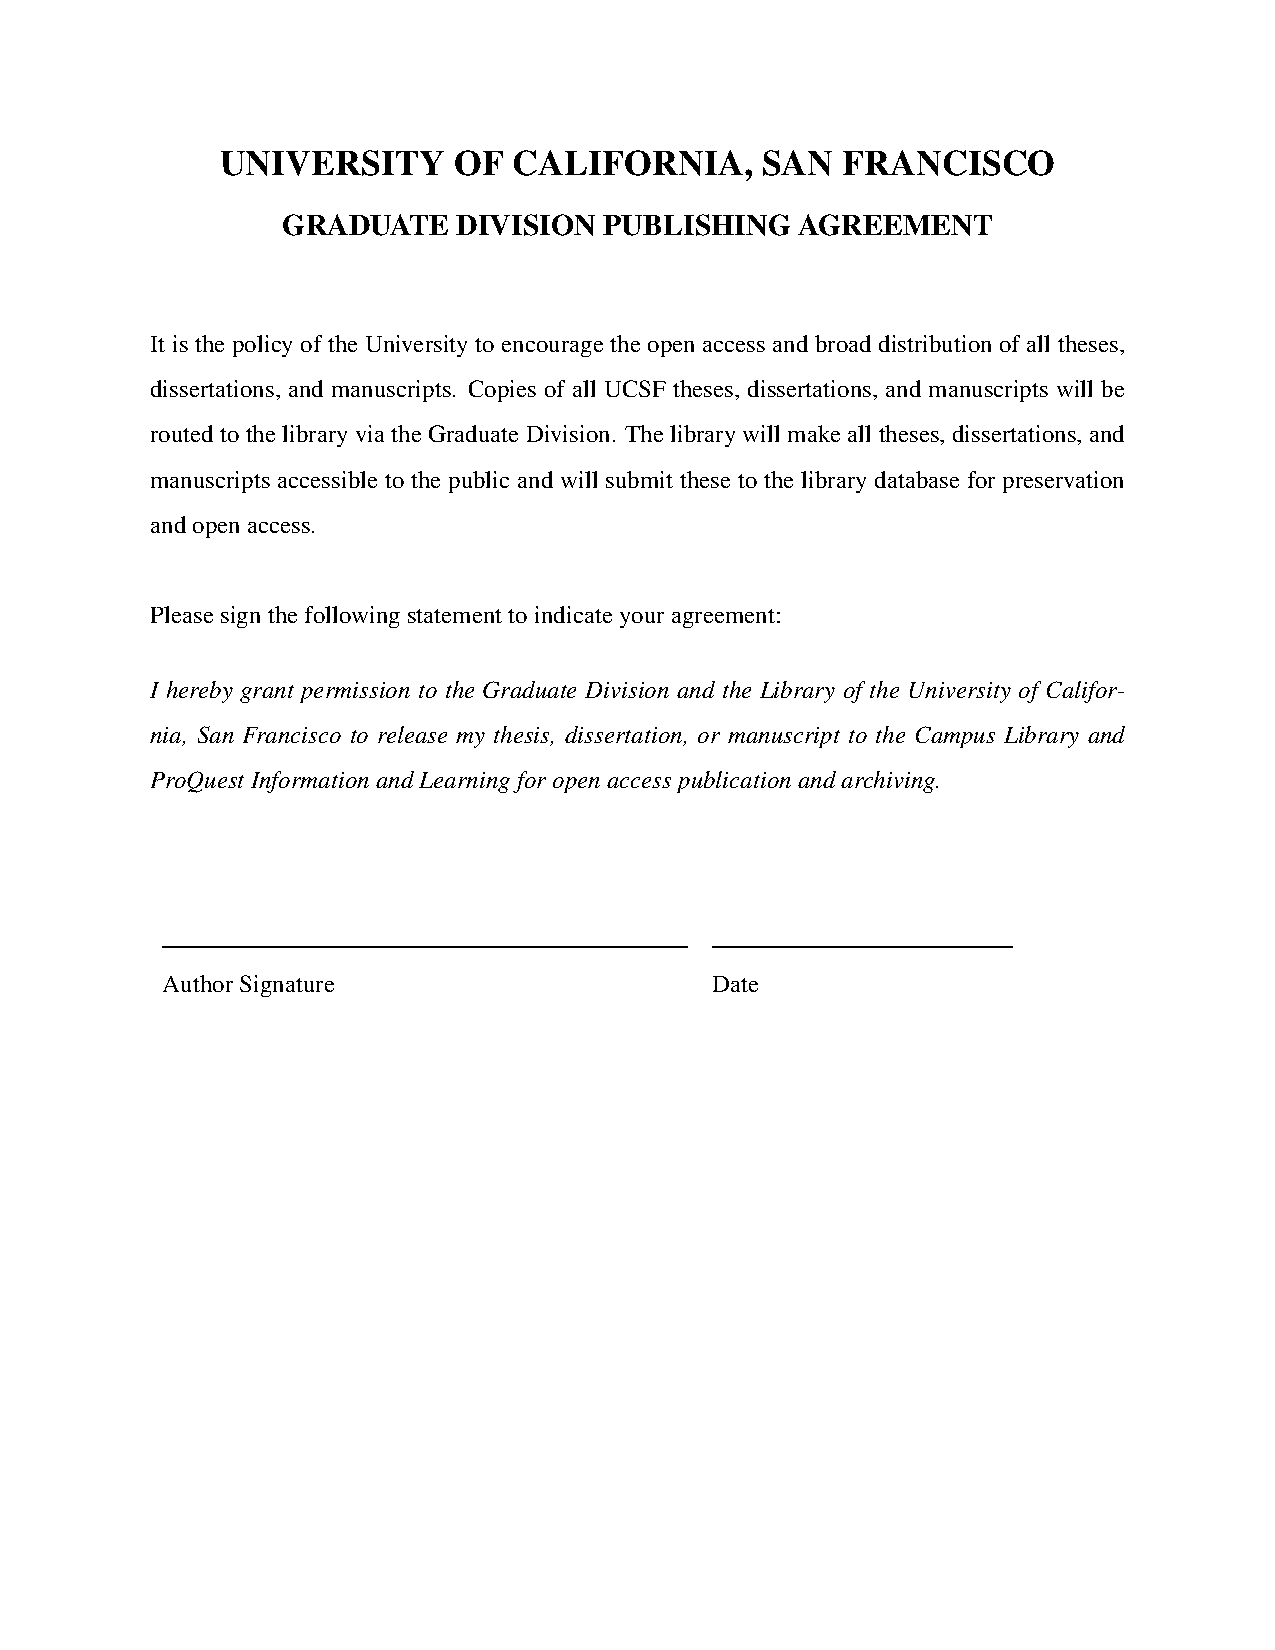
\includepdf[pages={1}, pagecommand={\thispagestyle{fancy}}]{publishing_agreement.pdf}

\end{document}
